\chapter{Results and Discussion} 
\label{Chapter5}

This chapter details the results and findings attained throughout this project. First, The feature selection results for each of the datasets used to train the 28 models are displayed. Then, the performance of each of the modelling techniques is displayed and discussed. This chapter then details if the alternative data features used throughout this project improved model performance and if the alternative features developed could be used to produce accurate loan default prediction models. Finally, the chapter displays the results of the McNemar's Chi Square tests used to compare the models developed.   

%%%%%%%%%%%%%%%%%%%%%%%%%%%%%%%%%%%%%%%

\section{Features Selection}

For each of the data category combinations shown in Section 4.1, RFE is used to identify the most relevant features, while cross validation is used to validate the optimal number of features. \\

Figures \ref{fig:sd}, \ref{fig:cb}, and \ref{fig:alt} are plots containing the number of features selected versus the model accuracy for datasets containing only sociodemographic, credit bureau, and alternative features respectively. Figure \ref{fig:all} displays the number of features selected against model accuracy for the dataset containing the features from all 3 data categories. \\

The figures display large variations in model accuracy based on the number of features used. This highlights the importance of feature selection.

\vspace{10 pt}

\begin{figure}[!htb]
\centering
  \begin{minipage}{0.5\textwidth}
    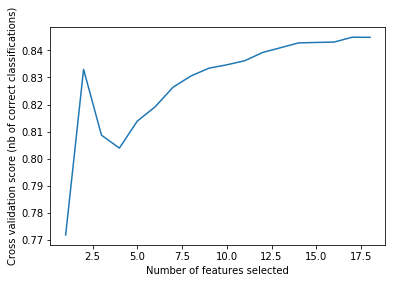
\includegraphics[width=\textwidth]{images/sd_only.png}
    \caption{Sociodemographic Variable Selection}
    \label{fig:sd}
  \end{minipage}%
  \begin{minipage}{0.5\textwidth}
    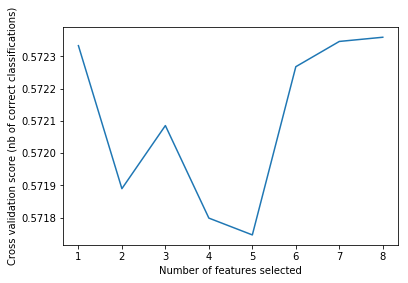
\includegraphics[width=\textwidth]{images/cb_only.png}
    \caption{Credit Bureau Variable Selection}
    \label{fig:cb}
  \end{minipage}
\end{figure}

\newpage

\vspace{10 pt}

\begin{figure}[!htb]
\centering
  \begin{minipage}{0.5\textwidth}
    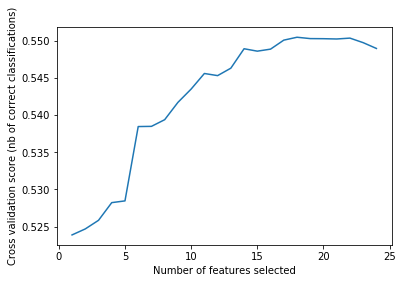
\includegraphics[width=\textwidth]{images/alt_only.png}
    \caption{Alternative Data Variable Selection}
    \label{fig:alt}
  \end{minipage}%
  \begin{minipage}{0.5\textwidth}
    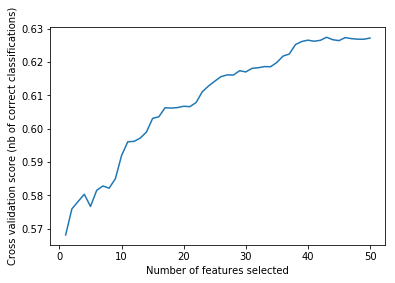
\includegraphics[width=\textwidth]{images/sd_cb_alt.png}
    \caption{Variable Selection for the All Datasets}
    \label{fig:all}
  \end{minipage}
\end{figure}

\vspace{10 pt}

Figure \ref{fig:sd} displays that when only SD features are used, there is a gradual increase in accuracy until 17 features are reached, then the accuracy plateaus. Figure \ref{fig:cb} displays that there is a decrease in accuracy when more CB features are added to the features space, until the number of features moves beyond 5. Figure \ref{fig:alt} displays that once the number of alternative data features moves beyond 8, there is either very little increase in accuracy or the accuracy decreases. Figure \ref{fig:all} displays that when using all data categories, model accuracy steadily improves when more feature dded to the feature space, until 43 features are in the feature space. \\

Table \ref{table:features retained} displays the feature selection results for all 7 data category combinations. The table provides the total number of features contained in each dataset, the number of features selected from the original datasets, and the names of the features that were deemed irrelevant (not selected). \\

The table highlights a mass drop of features when only CB and ALD features are used. This could indicate dependencies and collinearity between variables in that dataset, however the difference between the lowest and highest validation accuracies is last than 1\%.  \\

Furthermore, the Table validates the trends displayed in Figures \ref{fig:sd}, \ref{fig:cb}, \ref{fig:alt}, and \ref{fig:all}. This is particular evident in the ALD row, as it can be seen that a large number of features were deemed irrelevant. It is interesting that many of the ALD features not selected when only using ALD features, are deemed relevant when coupled with SD features.  \\

It can be noted that the variables are consistently removed by the RFE process. For example income is removed in the SD; SD and CB; SD and ALD; and SD, CB, and ALD datasets. The same pattern can be extended for many of the ALD and CB variables. \\

For each of the data category combinations, the various modelling techniques were trained and tested on the same dataset. The first modelling technique used is logistic regression. The cross-validated training results and the holdout results can be seen for this technique in the following section. \newpage


Table \ref{table:features retained} can be viewed below. 

\vspace{10pt}

\begin{longtable}{|p{3cm}|p{2cm}|p{2cm}|p{6cm}|} 
\hline
\multicolumn{1}{|p{3cm}|}{Dataset}
&\multicolumn{1}{|p{2cm}|}{Features}
&\multicolumn{1}{|p{2cm}|}{Selected Features}
&\multicolumn{1}{|p{6cm}|}{Features Not Selected}\\
\hline
SD & 18 & 16 & income   \\
\hline
CB & 8 & 8 &   \\
\hline
ALD & 24 & 8  & competitor count, gambling count, app count, max balance, max credit, max debit, min debit, insufficient funds,  successful payments, max successful loan payment, min  successful loan payment, unsuccessful payments, max unsuccessful loan payment, min unsuccessful loan payment, rejected loans, max loan amount \\
\hline
SD and CB & 26 & 21 & property status, time at employer , application time , application week , income \\
\hline
SD and ALD & 42 & 39 & income, competitor count, gambling count \\
\hline
CB and ALD & 32 & 3 &  open accounts by date, performing loans, paid loans, nonperforming loans, lost loans, missed payments, competitor count, banking count, news count, gambling count, VPN count, app count, device price, max balance, min balance, credit transactions, max credit, min credit, max debit, min debit, insufficient funds, successful payments, max successful loan payment, min successful loan payment, unsuccessful payments, max unsuccessful loan payment, min unsuccessful loan payment, rejected loans, max loan amount \\
\hline
SD, CB and ALD & 50 & 43 & application week, income, lost loans, competitor count, gambling count, insufficient funds, min unsuccessful loan payment\\
\hline
\caption{Feature Selection Results}
\label{table:features retained}
\end{longtable}

\vspace{10pt}

\newpage

%%%%%%%%%%%%%%%%%%%%%%%%%%%%%%%%%%%%%%%

\section{Logistic Regression}

Tables \ref{table:lr training} and \ref{table:lr test} respectively display the training and holdout results of the developed logistic regression models. \\

The holdout results displayed in Table \ref{table:lr test} highlight that the logistic regression models improved when the alternative features were added to the sociodemographic and credit bureau datasets. Furthermore, \ref{table:lr test} displays that the best performing model is trained using features from all three data categories. The model has the highest overall accuracy, repaid accuracy, F1 score, and AUC. The model developed using only credit bureau features and the model developed using the credit bureau and alternative features had high training and holdout default accuracy. However, the same models have low overall accuracy, repaid accuracy, F1 scores, and AUC values.  \\

The logistic regression model developed using only the alternative features does not perform well when classifying loans that were repaid. This can be seen in its low overall and repaid accuracies. The low F1 and AUC scores provide further validation that the model does not accurately predict the outcome of loans were repaid. \\

The holdout results displayed in Table \ref{table:lr test} closely align with the logistic regression results produced by \textcite{BigDataMicroFiance}. \\

There is very little discrepancy between the training and holdout model performance indicators for each logistic regression model. This provides a good indication that no over-fitting occurred during training. 

\vspace{10pt}

\begin{table}[H]
\begin{center}
\begin{tabular}{|c|c|c|c|c|c|} 
\hline
\multicolumn{1}{|c|}{Dataset}
&\multicolumn{1}{|c|}{Accuracy}
&\multicolumn{1}{|c|}{Repaid Accuracy}
&\multicolumn{1}{|c|}{Default Accuracy}
&\multicolumn{1}{|c|}{F1 Score}
&\multicolumn{1}{|c|}{AUC}\\
\hline
SD & 0.58 & 0.55 & 0.58 & 0.58 & 0.61    \\
\hline
CB & 0.57 & 0.39 & 0.76 & 0.57 & 0.60    \\
\hline
ALD & 0.54 & 0.46 & 0.62 & 0.54 & 0.56    \\
\hline
SD and CB & 0.60 & 0.60 & 0.61 & 0.60 & 0.65    \\
\hline
SD and ALD & 0.61 & 0.64 & 0.59 & 0.61 & 0.66    \\
\hline
CB and ALD & 0.58 & 0.44 & 0.75 & 0.59 & 0.61    \\
\hline
SD, CB and ALD & 0.63 & 0.62 & 0.64 & 0.63 & 0.68    \\
\hline
\end{tabular}
\end{center}
\caption{Logistic Regression Training Performance}
\label{table:lr training}
\end{table}

\vspace{10pt}

\begin{table}[H]
\begin{center}
\begin{tabular}{|c|c|c|c|c|c|} 
\hline
\multicolumn{1}{|c|}{Dataset}
&\multicolumn{1}{|c|}{Accuracy}
&\multicolumn{1}{|c|}{Repaid Accuracy}
&\multicolumn{1}{|c|}{Default Accuracy}
&\multicolumn{1}{|c|}{F1 Score}
&\multicolumn{1}{|c|}{AUC}\\
\hline
SD & 0.61 & 0.62 & 0.55 & 0.61 & 0.63    \\
\hline
CB & 0.48 & 0.40 & 0.75 & 0.48 & 0.62    \\
\hline
ALD & 0.50 & 0.47 & 0.64 & 0.51 & 0.57    \\
\hline
SD and CB & 0.61 & 0.61 & 0.62 & 0.61 & 0.65    \\
\hline
SD and ALD & 0.63 & 0.64 & 0.59 & 0.63 & 0.66    \\
\hline
CB and ALD & 0.51 & 0.43 & 0.73 & 0.53 & 0.62    \\
\hline
SD, CB and ALD & 0.64 & 0.64 & 0.63 & 0.63 & 0.68    \\
\hline
\end{tabular}
\end{center}
\caption{Logistic Regression Holdout Performance}
\label{table:lr test}
\end{table}

\vspace{10pt}

%%%%%%%%%%%%%%%%%%%%%%%%%%%%%%%%%%%%%%%


\section{Random Forest}

Tables \ref{table:rf training} and \ref{table:rf test} respectively display the cross validation and holdout results of random forests models developed throughout this project. \\

It can be seen that the random forest models produce better training performance indicators than the logistic regression models - shown in Table \ref{table:lr training}. The holdout default accuarcies of the random forest models are, at times, significantly  lower than the holdout default accuarcies of the logistic regression models - shown in Table \ref{table:lr test}. This is due to a combination of effects of SMOTE and that Random forest models, like other ensemble techniques, make use of classical sub-sampling methods \parencite{Minority}. \\

SMOTE is only applied to training datasets of the developed models, meaning that the synthetic obvserabtaions are only generated from the data points in the training data and not from data points on the test data. Variation in the minority class observations leads to differences between the observations in the training and test data. Therefore the RF models struggle to identify minority class observations in the holdout sets \parencite{NNShen}. \\

The sub-sampling performed when the RF models are trained can result in a common data distribution shared by all base-classifiers. This can result in the loss of important information which in turn results in the trained models poorly identifying the minority class observations contained within the holdout sets \parencite{Minority}. \\

\vspace{10pt}

\begin{table}[H]
\begin{center}
\begin{tabular}{|c|c|c|c|c|c|} 
\hline
\multicolumn{1}{|c|}{Dataset}
&\multicolumn{1}{|c|}{Accuracy}
&\multicolumn{1}{|c|}{Repaid Accuracy}
&\multicolumn{1}{|c|}{Default Accuracy}
&\multicolumn{1}{|c|}{F1 Score}
&\multicolumn{1}{|c|}{AUC}\\
\hline
SD & 0.81 & 0.82 & 0.81 & 0.82 & 0.83    \\
\hline
CB & 0.63 & 0.53 & 0.74 & 0.63 & 0.68    \\
\hline
ALD & 0.71 & 0.74 & 0.69 & 0.71 & 0.80    \\
\hline
SD and CB & 0.83 & 0.83 & 0.83 & 0.83 & 0.88    \\
\hline
SD and ALD & 0.85 & 0.86 & 0.85 & 0.85 & 0.92    \\
\hline
CB and ALD & 0.69 & 0.68 & 0.71 & 0.70 & 0.78    \\
\hline
SD, CB and ALD & 0.87 & 0.87 & 0.87 & 0.87 & 0.93    \\
\hline
\end{tabular}
\end{center}
\caption{Random Forest Training Performance}
\label{table:rf training}
\end{table}

\vspace{10pt}

\begin{table}[H]
\begin{center}
\begin{tabular}{|c|c|c|c|c|c|} 
\hline
\multicolumn{1}{|c|}{Dataset}
&\multicolumn{1}{|c|}{Accuracy}
&\multicolumn{1}{|c|}{Repaid Accuracy}
&\multicolumn{1}{|c|}{Default Accuracy}
&\multicolumn{1}{|c|}{F1 Score}
&\multicolumn{1}{|c|}{AUC}\\
\hline
SD & 0.71 & 0.81 & 0.37 & 0.70 & 0.60    \\
\hline
CB & 0.56 & 0.52 & 0.68 & 0.56 & 0.63    \\
\hline
ALD & 0.66 & 0.72 & 0.44 & 0.66 & 0.62    \\
\hline
SD and CB & 0.73 & 0.83 & 0.39 & 0.73 & 0.66    \\
\hline
SD and ALD & 0.79 & 0.86 & 0.53 & 0.78 & 0.80    \\
\hline
CB and ALD & 0.64 & 0.68 & 0.47 & 0.64 & 0.60    \\
\hline
SD, CB and ALD & 0.80 & 0.87 & 0.54 & 0.79 & 0.81    \\
\hline
\end{tabular}
\end{center}
\caption{Random Forest Holdout Performance}
\label{table:rf test}
\end{table}

\vspace{10pt}


The most accurate RF model is trained using features from all three data categories. Furthermore, when alternative features were added to both the datasets containing the sociodemographic and the credit bureau features the performance of the random forest models improve. This can be seen in accuracy, repaid accuracy, F1 score, and AUC values displayed in Table \ref{table:rf test}. Similarly to the logistic regression model containing only credit bureau features, the respective random forest model performs better than other other random forest models when identifying loans that were not repaid.  


%%%%%%%%%%%%%%%%%%%%%%%%%%%%%%%%%%%%%%%


\section{Extreme Gradient Boosting}

The third modelling technique used is XGBoost. Tables \ref{table:xgb training} and \ref{table:xgb test} display the training and holdout results of the 7 XGBoost models developed throughout this project. \\

Table \ref{table:xgb test} displays that in general, the XGBoost models outperform their respective logistic regression and random forest models. It can be seen from both XGBoost tables that the test default accuracy is often significantly lower than the training default accuracy. This trend is seen in the random forest models and occurs in the XGBoost models for the same reasons that it occurs in the random forest models (the effects of SMOTE and sub-sampling). \\ 

Table \ref{table:xgb test} highlights the alternative features improve the overall accuracy, repaid accuracy, F1 score, AUC of the XGBoost models when added to data containing sociodemographic and credit bureau features. 

\vspace{10pt}

\begin{table}[H]
\begin{center}
\begin{tabular}{|c|c|c|c|c|c|} 
\hline
\multicolumn{1}{|c|}{Dataset}
&\multicolumn{1}{|c|}{Accuracy}
&\multicolumn{1}{|c|}{Repaid Accuracy}
&\multicolumn{1}{|c|}{Default Accuracy}
&\multicolumn{1}{|c|}{F1 Score}
&\multicolumn{1}{|c|}{AUC}\\
\hline
SD & 0.83 & 0.82 & 0.84 & 0.83 & 0.91    \\
\hline
CB & 0.65 & 0.56 & 0.75 & 0.63 & 0.72    \\
\hline
ALD & 0.80 & 0.79 & 0.81 & 0.80 & 0.88    \\
\hline
SD and CB & 0.82 & 0.78 & 0.85 & 0.82 & 0.91    \\
\hline
SD and ALD & 0.91 & 0.89 & 0.93 & 0.91 & 0.96    \\
\hline
CB and ALD & 0.74 & 0.76 & 0.72 & 0.74 & 0.82    \\
\hline
SD, CB and ALD & 0.90 & 0.93 & 0.92 & 0.91 & 0.98    \\
\hline
\end{tabular}
\end{center}
\caption{XGBoost Training Performance}
\label{table:xgb training}
\end{table}

\vspace{10pt}

\begin{table}[H]
\begin{center}
\begin{tabular}{|c|c|c|c|c|c|} 
\hline
\multicolumn{1}{|c|}{Dataset}
&\multicolumn{1}{|c|}{Accuracy}
&\multicolumn{1}{|c|}{Repaid Accuracy}
&\multicolumn{1}{|c|}{Default Accuracy}
&\multicolumn{1}{|c|}{F1 Score}
&\multicolumn{1}{|c|}{AUC}\\
\hline
SD & 0.71 & 0.81 & 0.38 & 0.72 & 0.62    \\
\hline
CB & 0.59 & 0.55 & 0.64 & 0.57 & 0.63    \\
\hline
ALD & 0.69 & 0.78 & 0.40 & 0.69 & 0.63    \\
\hline
SD and CB & 0.71 & 0.78 & 0.46 & 0.70 & 0.68    \\
\hline
SD and ALD & 0.82 & 0.86 & 0.66 & 0.81 & 0.85    \\
\hline
CB and ALD & 0.68 & 0.77 & 0.41 & 0.69 & 0.62    \\
\hline
SD, CB and ALD & 0.84 & 0.88 & 0.68 & 0.82 & 0.86    \\
\hline
\end{tabular}
\end{center}
\caption{XGBoost Holdout Performance}
\label{table:xgb test}
\end{table}

\vspace{10pt}

Similarly to both the logistic regression and random forest techniques, the best performing XGBoost model is trained on the dataset containing features from all three data categories. This model is subsequently the best performing model out of all 28 developed throughout this project, therefore this model is further analysed by assessing its ROC curves and the impact of certain features on the model. 


\subsubsection{ROC Curves}


Figures \ref{fig:xgb_tr} and \ref{fig:xgb_te} display the training and test ROC curves for the best performing XGBoost model. The decrease  default accuracy from training to testing is reflected in the figures.

\vspace{10 pt}

\begin{figure}[!htb]
\centering
  \begin{minipage}{0.5\textwidth}
    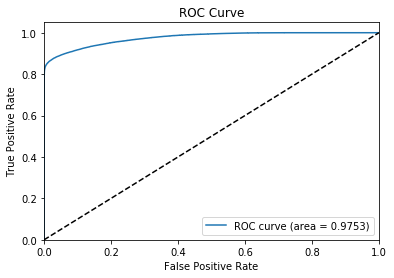
\includegraphics[width=\textwidth]{images/XGB_TR_AUC.png}
    \caption{XGBoost Training ROC}
    \label{fig:xgb_tr}
  \end{minipage}%
  \begin{minipage}{0.5\textwidth}
    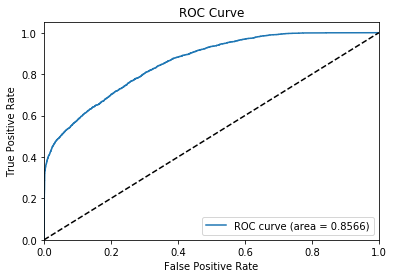
\includegraphics[width=\textwidth]{images/XGB_TE_AUC.png}
    \caption{XGBoost Holdout ROC}
    \label{fig:xgb_te}
  \end{minipage}
\end{figure}


\subsubsection{Feature Impact}

The SHapley Additive exPlanation (SHAP) values for the ten most important features of the best performing XGBoost model can be seen in Figure \ref{fig:xgb_feats}. SHAP values show how much each feature contributes, either positively or negatively, to the target variable. The each dot in the plot represents a training observation. The plot demonstrates feature importance, the impact of an observation on the final prediction, the relative value of feature for an observation, and the correlation between features and the final prediction \parencite{SHAP}. 

\vspace{10 pt}

\begin{figure}[!htb]
\centering
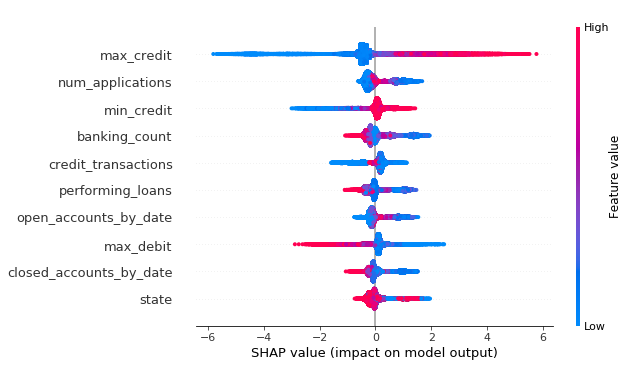
\includegraphics[width=0.6\textwidth]{images/xgb_feats.png}
\caption{SHAP Values of Best Performing XGBoost Model}
\label{fig:xgb_feats}
\end{figure}

\vspace{10 pt}

The features are ranked in descending order of importance in Figure \ref{fig:xgb_feats}. For example the maximum credit extracted from loan applicants' sms messages - an alternative feature - is the most important feature used in the model. Furthermore, we can see the impact the maximum credit feature has on the model. The lower the maximum credit value, the more negative its impact is on the model. This means that the lower an applicant's extracted maximum credit is, the more likely the model is to classify the application into the defaulting class. We can see that this is converse to the number of applications made by a client prior to their current loan application The lower the number of applications, the more positive the feature's impact is on the model. \\


\subsubsection{Using only ALD Features}

The XGBoost model trained using only alternative features had an overall test accuracy of 66\%, a repaid accuracy of 72\%, an f1 score of 0.66, and an AUC of 0.62. These would all indicate the model could be used to accurately predict the outcome of a loan. However, the default of the model accuracy was only 44\%. Meaning that the model does not identify loans that are likely to not be repaid well. \\

The final technique explored during this project is Neural Networks. The following section displays the features of the multi-layer perceptron networks developed.  

%%%%%%%%%%%%%%%%%%%%%%%%%%%%%%%%%%%%%%%


\section{Neural Networks}

The training and holdout results of the 7 MLP models developed throughout this projected can be seen in Tables \ref{table:NN training} and \ref{table:NN test}.  \\

The MLP models showed slightly different trends to the other modelling techniques. The best performing model based upon overall accuracy, AUC and F1 score is the model trained using features from all three data categories. However, when the alternative data features were add to the sociodemographic and credit bureau datasets, model performance across all five measures did not improve.    

\vspace{10pt}

\begin{table}[H]
\begin{center}
\begin{tabular}{|c|c|c|c|c|c|} 
\hline
\multicolumn{1}{|c|}{Dataset}
&\multicolumn{1}{|c|}{Accuracy}
&\multicolumn{1}{|c|}{Repaid Accuracy}
&\multicolumn{1}{|c|}{Default Accuracy}
&\multicolumn{1}{|c|}{F1 Score}
&\multicolumn{1}{|c|}{AUC}\\
\hline
SD & 0.60 & 0.73 & 0.44 & 0.59 & 0.63    \\
\hline
CB & 0.58 & 0.79 & 0.35 & 0.57 & 0.61    \\
\hline
ALD & 0.51 & 0.54 & 0.47 & 0.50 & 0.52    \\
\hline
SD and CB & 0.64 & 0.53 & 0.72 & 0.64 & 0.68    \\
\hline
SD and ALD & 0.67 & 0.52 & 0.83 & 0.67 & 0.74    \\
\hline
CB and ALD & 0.59 & 0.42 & 0.75 & 0.59 & 0.62    \\
\hline
SD, CB and ALD & 0.71 & 0.73 & 0.68 & 0.71 & 0.78    \\
\hline
\end{tabular}
\end{center}
\caption{Neural Network Training Performance}
\label{table:NN training}
\end{table}

\vspace{10pt}

\begin{table}[H]
\begin{center}
\begin{tabular}{|c|c|c|c|c|c|} 
\hline
\multicolumn{1}{|c|}{Dataset}
&\multicolumn{1}{|c|}{Accuracy}
&\multicolumn{1}{|c|}{Repaid Accuracy}
&\multicolumn{1}{|c|}{Default Accuracy}
&\multicolumn{1}{|c|}{F1 Score}
&\multicolumn{1}{|c|}{AUC}\\
\hline
SD & 0.65 & 0.77 & 0.43 & 0.66 & 0.64    \\
\hline
CB & 0.70 & 0.79 & 0.39 & 0.70 & 0.63    \\
\hline
ALD & 0.53 & 0.54 & 0.52 & 0.53 & 0.51    \\
\hline
SD and CB & 0.68 & 0.55 & 0.73 & 0.67 & 0.68    \\
\hline
SD and ALD & 0.60 & 0.52 & 0.80 & 0.60 & 0.73    \\
\hline
CB and ALD & 0.58 & 0.53 & 0.47 & 0.58 & 0.62    \\
\hline
SD, CB and ALD & 0.70 & 0.74 & 0.66 & 0.71 & 0.73    \\
\hline
\end{tabular}
\end{center}
\caption{Neural Network Holdout Performance}
\label{table:NN test}
\end{table}

\vspace{10pt}

The MLP models developed throughout this project showed similar patterns to those developed by \textcite{NNWest}. The models generally had a higher repaid accuracy than a default accuracy. However, the overall accuracies achieved by the models developed by \textcite{NNWest} were significantly higher than those developed throughout this project. \\

The final step in the testing process was to statically compare the performance of the models across each of the 7 datasets. The results of the tests are shown in the following section. 

%%%%%%%%%%%%%%%%%%%%%%%%%%%%%%%%%%%%%%%

\section{Model Comparison}

The performance indicators displayed in the tables that preceded this section each model indicate that the performance of the models improved when alternative data features were added to sociodemographic and credit bureau datasets (the only exception were the NN models). Furthermore, the optimal model developed across all 4 techniques used sociodemographic, credit bureau, and alternative data features. The random forest and XGBoost models developed using only alternative features displayed good overall accuracy, high repaid accuracy, good F1 scores, and good AUC values. However, both models display low default accuracy. The logistic regression and MLP models developed using only alternative features display poor overall performance. \\ 

The final test performed on the models is McNemar's Chi Square test, which tests if there is a significant difference between two models trained on the same sample. The test is used to compare each technique against all other techniques for all 7 data category combinations. Table \ref{table:Mcnemar} displays the results of the  McNemar's tests conducted. The techniques compared are seen on the left hand side of the table while the data category combinations are shown along the top of the table. \\

The null hypothesis of the McNemar's Chi Square test states that the models compared are not significantly different. The values in Table \ref{table:Mcnemar} are true is the test resulted in the null hypothesis is accepted - the models are not significantly different - and are false if the null hypothesis is rejected - the models are significantly different. 

\vspace{10pt}

\begin{table}[H]
\begin{center}
\begin{tabular}{|c|c|c|c|c|c|c|c|} 
\hline
\multicolumn{1}{|c|}{Techniques}
&\multicolumn{1}{|c|}{SD}
&\multicolumn{1}{|c|}{CB}
&\multicolumn{1}{|c|}{ALD}
&\multicolumn{1}{|c|}{SD, CB}
&\multicolumn{1}{|c|}{SD, ALD}
&\multicolumn{1}{|c|}{CB, ALD}
&\multicolumn{1}{|c|}{SD, CB, ALD}\\
\hline
LR - RF & false & false & false  & false & false &  false &  false \\
\hline
LR - XGB & false & false & false & false  & false & false & false \\
\hline
LR - MLP & false & false  & false & false & false & false & false \\
\hline
RF - XGB & false & false & false & true & false & false &  false \\
\hline
RF - MLP & true & false & false & false & false & false & false  \\
\hline
XGB - MLP & true & false & false & false & false & false &  false \\
\hline
\end{tabular}
\end{center}
\caption{McNemar's Chi Square Tests}
\label{table:Mcnemar}
\end{table}

\vspace{10pt}

We can see from Table \ref{table:Mcnemar} that the other than the RF and MLP, and the XGBoost and MLP models trained used only sociodemographic features the models are deemed significantly different. This means that their model performance indicators can be used to dictate which models perform best. \\

Across all data category combinations - other than the combination that uses only credit bureau variables - the XGBoost technique produces the model with the highest overall accuracy repaid accuracy, F1 score, and AUC value (only considering holdout values). The XGBoost technique does not consistently produce the highest default accuracy. The XGBoost model developed using all three data category combinations performs the best across all five performance indicators. \\

\section{Summary of Modelling Results}

This chapters displays the cross-validated training results and the holdout results of each of the models developed throughout this project. The alternative features developed during this project are found to improve the performance of loan default prediction models when added to sociodemographic: for the logistic regression, random forest, and XGBoost techniques. For all 4 techniques used the most accurate model is trained on a dataset contain sociodemographic, credit bureau, and alternative features. Models developed only using the alternative features did not perform well. The best performing model developed using only alternative features used XGBoosting, however even that model has a low default accuracy. This indicates that the alternative features used throughout this project cannot solely be used to develop a loan prediction model. Finally, the model were proven to be significantly different using McNemar's Chi Squared Test with 1 degree of freedom. The consistently best performing technique used for loan default prediction in this project is XGBoosting. \\

The final chapter of this project summarises the conclusions and findings of the research. 